\chapter{Proprietà di Correttezza e di Verifica}

\section{Java Pathfinder}
Per il model checking del sistema è stata utilizzata anche la libreria Java Pathfinder.\newline
Java Pathfinder è un sistema per verificare i programmi eseguibili bytecode Java. JPF è stato sviluppato presso il Centro ricerche Ames della NASA e aperto nel 2005.\newline
Grazie a Java Pathfinder è possibile grazie ad una semplice riga di comando verificare se esistono stati del programma in cui si verificano eccezioni o situazioni indesiderate.\newline
Nello specifico, è possibile anche verificare aspetti relativi alla concorrenza.\newline
\begin{figure}[H]
	\begin{center}
		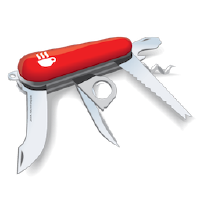
\includegraphics[width=0.25\linewidth]{img/JavaPathFinder.png}
		\label{fig:jpflogo}
		\caption{Logo di JPF}
	\end{center}
\end{figure}

\subsection{Modalità di utilizzo}
Per utilizzare Java Pathfinder è stato necessario creare una nuova classe eseguibile, denominata \textit{AppConcurrentJPF}.\newline Per eseguire Java Pathfinder utilizzando la corretta configurazione è necessario lanciare il comando:
\begin{lstlisting}[language=bash, caption="Comando utilizzato per eseguire Java Pathfinder"]
java -jar ../JPF/jpf-core/build/RunJPF.jar +classpath=build/classes/java/main jpf.controller.apps.AppConcurrentJPF
\end{lstlisting}
Grazie a Gradle è stato possibile automatizzare ancora di più questo processo creando un apposito task nel file di configurazione \textit{build.gradle}:
\begin{lstlisting}[language=Java, caption="Gradle Task utilizzato per eseguire Java Pathfinder"]

task("runJPF", JavaExec::class) {
    main = "jpf.controller.apps.AppConcurrentJPF"
    classpath = sourceSets["main"].runtimeClasspath
    doLast {
        exec {
            commandLine = listOf("java", "-jar", "../JPF/jpf-core/build/RunJPF.jar", "+classpath=build/classes/java/main", "jpf.controller.apps.AppConcurrentJPF")
        }
    }
}
\end{lstlisting}
Eseguendo da terminale il comando \textit{"gradle runJPF"} verrà eseguita l'operazione di build e di esecuzione della classe \textit{"AppConcurrentJPF"}, seguita dalla verifica da parte di JPF (equivalente ad eseguire il comando).

\subsection{Organizzazione del progetto}

Oltre alla classe AppConcurrentJPF in realtà è stato in realtà necessario astrarre e semplificare alcuni meccanismi del sistema per permettere una più semplice verifica del sistema.\newline
È stato quindi necessario creare un package denominato \textit{jpf} il cui scopo è contenere implementazioni semplificate di alcune classi che utilizza \textit{AppConcurrent}. La struttura del package e la medesima del progetto nella sua completezza, contiene i sotto-package model e controller i quali contengono a loro volta i sorgenti delle classi che sono state sensibilmente modificate.\newline
La struttura di \textit{AppConcurrentJPF} è a tutti gli effetti identica a quella di \textit{AppConcurrent}, ma alcune classi dipendenti sono state modificate per semplicità.
\begin{warn}[ATTENZIONE:]
Alcune delle metodologie utilizzata per effettuare il model checking che verranno illustrate a breve non sono meccanismi che rappresentano lo stato dell'arte nella programmazione, come ad esempio, inserire dei valori hard-coded all'interno del codice.\newline
L'utilizzo di questi metodi è però stato necessario a causa della natura di Java Pathfinder. La libreria presenta infatti alcune lacune di compatibilità evidenti, e non è possibile effettuare un model checking pulito senza apportare le modifiche che seguono.
\end{warn}
In particolare:
\begin{itemize}
    \item La fase di lettura del file delle parole da ignorare utilizza un \textit{BufferedReader}. Java Pathfinder non è stato in grado in nessun modo di oltrepassare la fase di lettura del file. Impostando la dimensione del buffer al valore predefinito veniva lanciata un'eccezione di tipo \textit{BufferOverflowException}, impostandola un valore più basso l'eccezione cambiava in \textit{IndexOutOfBoundException}. Il problema è stato risolto rimuovendo il processo di lettura da file (il quale non era nemmeno un aspetto relativo alla concorrenza) e creando una classe apposita \textit{IgnoredWordsJPF} la quale restituisce un Set di parole da ignorare inserite hard-coded.
    \item In nessun modo è stato possibile fare model checking includendo anche classi della libreria \textit{PDFBox}.\newline
    Anche includendo il file jar della libreria nel classpath (nel comando utilizzato per lanciare JPF) il problema si sposta sul non trovare dipendenze della libreria stessa. Includendo le dipendenze si presentano errori molto più a basso livello, i quali sono quasi impossibili da risolvere, anche perché molto probabilmente relativi a come sono state implementate le librerie.\newline
    La soluzione è stata creare una nuova classe \textit{ReadFileTaskJPF} che non utilizzasse la libreria, ma che invece che leggere frasi da pagine di un documento PDF le recuperasse da un oggetto in grado di generarne alcune pseudo-casualmente.
    \item Alcuni degli argomenti (la directory dei file pdf, il path del file contenente le parole da ignorare e il numero di parole con più occorrenza da mostrare al termine dell'esecuzione) vengono ancora utilizzati, anche se alcuni vengono trattati in modo diverso. Tutti e tre questi valori sono inseriti in maniera hard-coded, non ha infatti senso utilizzare valori sbagliati per questo tipo di testing. Il numero di parole da mostrare al termine del programma mantiene la sua funzione, il nome del file delle parole ignorate non viene utilizzato, mentre il path della cartella che contiene i PDF viene utilizzata solo per leggere il numero di file all'interno della cartella. La lettura del file è "simulata", vengono infatti comunque creati \textit{\#n} task di tipo \textit{ReadFileTaskJPF} (dove \textit{\#n} è il numero di documenti nella cartella), ma il testo al loro interno viene recuperato dall'oggetto illustrato al punto precedente invece che dai PDF stessi.
\end{itemize}

\subsection{Eccezioni e problemi riscontrati}
Non sono stati riscontrati particolari problemi relativi alla concorrenza.\newline
Java Pathfinder è stato comunque utile in quanto è riuscito ad identificare le possibili seguenti eccezioni:
\begin{itemize}
\item \textbf{NullPointerException}: Si trattava di un'eccezione non gestita correttamente durante la creazione dell'oggetto che rappresenta la cartella in cui sono contenuti i file PDF;
\item \textbf{ClassCastException}: L'eccezione veniva lanciata nel momento in cui veniva richiamato il metodo \textit{Collections.toSet()} da parte di uno Stream. Creare il set usando un ciclo foreach ha risolto il problema;
\begin{info}
I metodi utilizzati dalla classe \textit{Collections} per convertire uno Stream ad una struttura dati a scelta è un meccanismo di Java particolarmente utilizzato, ma JPF lo ha definito comunque come fonte di eccezione in ogni punto in cui è stato utilizzato.
I metodi sono stati riscritti in modo da non utilizzare Stream, utilizzando un approccio più iterativo a soli fini di verificare la correttezza complessiva del sistema.
L'utilizzo di Stream è in alcuni casi specifici ritenuto più efficiente e riteniamo che una volta effettuato il model checking sarebbe più opportuno utilizzare la versione più efficiente e più di alto livello possibile.
\end{info}
\item \textbf{BufferOverflowException}: L'eccezione veniva lanciata durante la fase di caricamento del file delle parole ignorate. Rimuovere la lettura da file e inserire stringhe hard-coded ha risolto il problema.
\end{itemize}
\subsection{Resoconto sull'utilizzo di Java Pathfinder}

Il risultato restituito da Java Pathfinder dopo aver risolto tutte le eccezioni sopra riportate è stato il desiderato:

\begin{figure}[H]
	\begin{center}
		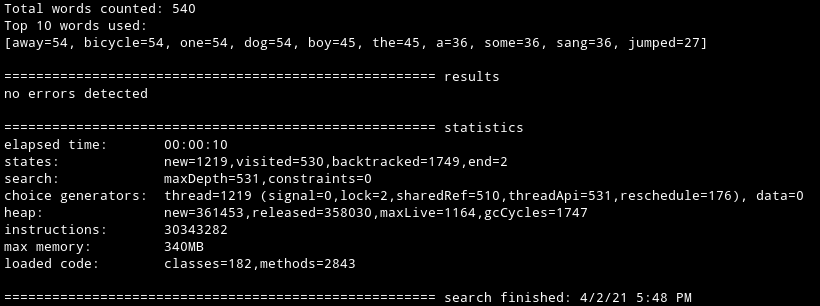
\includegraphics[width=\linewidth]{img/jpf_result.png}
		\label{fig:jpfResult}
		\caption{Risultato finale ottenuto utilizzando JPF}
	\end{center}
\end{figure}

\section{Tina 3.6}
Per verificare la correttezza di alcune logiche temporali nella Rete di Petri è stato utilizzato il tool Tina 3.6.\newline
Tina permette di modellare una Rete di Petri e di costruire il suo Marking Graph.
\begin{figure}[H]
	\begin{center}
		
\includegraphics[width=0.2\linewidth]{img/tina.png}
		\label{fig:tina}
		\caption{Logo di Tina}
	\end{center}
\end{figure}
\begin{info}[INFO:]
Un Marking Graph è una rete di Petri in cui ogni piazza ha esattamente un arco uscente ed uno entrante. Questo significa che non ci possono essere conflitti, ma può comunque esserci concorrenza.
\end{info}
Tina permette a partire da una rete di Petri di verificare proprietà esprimibili per esempio tramite logiche temporali.
\newline
Grazie al tool verificheremo che le seguenti proprietà valgano:
\begin{itemize}
    \item
    $\square$ ( $\lnot$ map token $\Rightarrow$ $\lozenge$ final map token) : \textbf{TRUE} \newline
    È sempre vero che se si acquisisce il token per entrare in sezione critica, prima o poi questo verrà rilasciato.

\item $\square$(pdf in path $\Rightarrow$ $\lozenge$file read task) : \textbf{TRUE} \newline
    È sempre vero che se ci sono documenti PDF disponibili non ancora elaborati nel path specificato, allora verrà prima o poi creato un \textit {file read task} per tale file.

    \item $\square$(file read task $\Rightarrow$ $\lozenge$($\lnot$final map token)):\textbf{TRUE} \newline
    È sempre vero che se esiste almeno un file read task disponibile, allora questo prima o poi acquisirà il final map token per accedere alla sezione critica.

    \item  pdf in path $U$ ($\lnot$ pdf in path): \textbf{TRUE} \newline
    Tutti i documenti nel path prima o poi verranno elaborati, finché non saranno esauriti.

    \item $\bigcirc$(pdf in path $\wedge$ workers): \textbf{TRUE} \newline
    Verranno istanziati i workers ed identificati i file nel path nel secondo mondo temporale.

    \item $\square$($\lnot$workers $\Rightarrow$ $\lozenge$workers): \textbf{TRUE} \newline
    È sempre vero che non ci sono workers disponibili, prima o poi ce ne saranno.

    \item $\square$workers: \textbf{FALSE} \newline
    Non sono sempre disponibili workers.

    \item $\square$final map token: \textbf{FALSE} \newline
    È sempre vero che non si è mai in sezione critica.

\end{itemize}

% Identificazione di proprietà di correttezza e verifica (JPF e/o TLA+).
